\section{Experiments}
\label{sec:4}
\subsection{ModelNet40 dataset}
In our experiments we used well known data set of 3D objects ModelNet40.
It is a subset of 40 classes of larger data set called ModelNet \cite{wu20153d} that contains different 3D CAD models in OFF format.

The total size of ModelNet40 data set $12311$.
The data set is split into training and test subsets, their sizes are $9843$ and $2468$ correspondingly.
The data set is not balanced.
Number of samples per class vary: from 64 to 889, see Figure \ref{fig:modelnet_classes}.

\begin{figure}
	\centering
    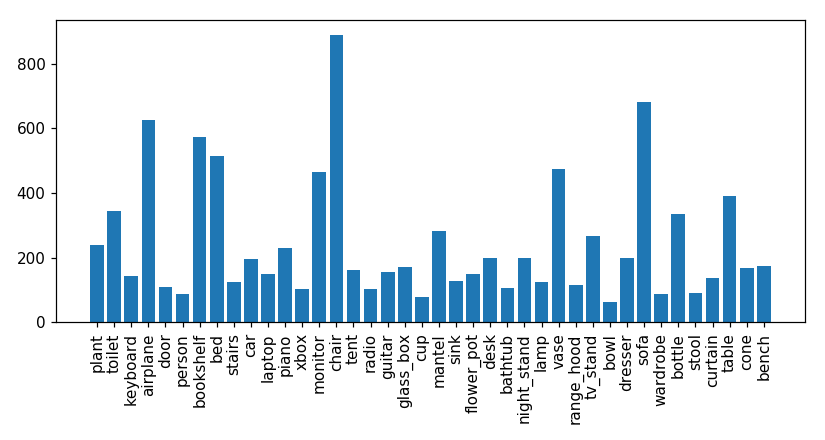
\includegraphics[width=\textwidth]{Figures/shape_retrieval/modelnet_classes.png}
    \caption{ModelNet40 data set: distribution of samples per class.}
    \label{fig:modelnet_classes}
\end{figure}

\subsection{Implementation details}
To demonstrate the impact that the triplet based training has on the performance of CNN descriptors
we use a deep network architecture shown in a Table~\ref{tab:net-architecture}. This network was implemented in PySparseConvNet, which is our modification of the SparseConvNet library \cite{graham2014spatially}. Besides new loss functions PySparseConvNet can be accessed from Python for a more interactive usage.

When forming a triplet for training we choose uniformly randomly a positive pair of objects from one class
and select a negative sample uniformly randomly from one of other classes.

For the optimization we use the SGD \cite{bottou-tricks-2012}, and the training is done
\begin{itemize}
\item in batches of size from $45$ to $90$ depending on a GPU video memory,
\item with a learning rate of $0.002$,
\item and a momentum equal to $0.99$.
\end{itemize}
Training can take up to a week on a server with advanced GPU, such as NVIDIA Titan X or GTX980ti.

\begin{figure}
\centering
\begin{tabular}{ccccc}
  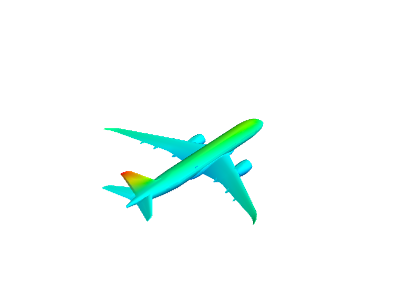
\includegraphics[width=0.19\columnwidth]{Figures/shape_retrieval/pic_airplane_solid.png} &
  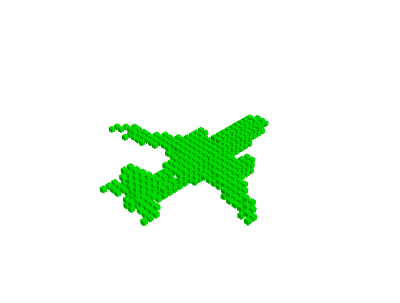
\includegraphics[width=0.19\columnwidth]{Figures/shape_retrieval/pic_airplane_30_solid.png} &
  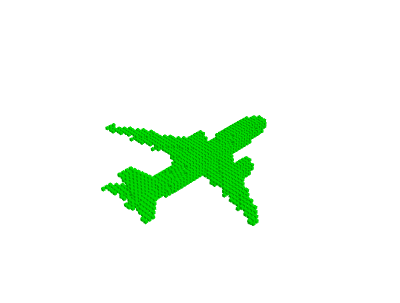
\includegraphics[width=0.19\columnwidth]{Figures/shape_retrieval/pic_airplane_50_solid.png} &
  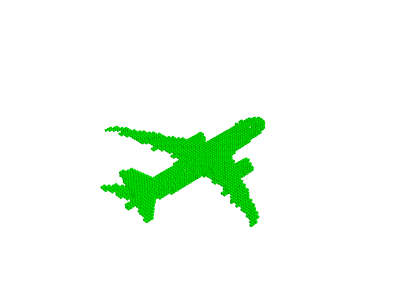
\includegraphics[width=0.19\columnwidth]{Figures/shape_retrieval/pic_airplane_70_solid.png} &
  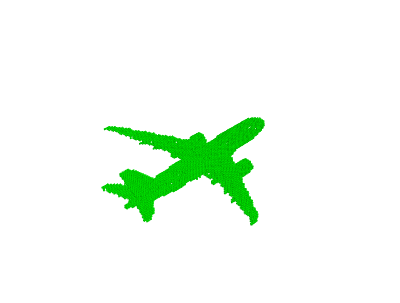
\includegraphics[width=0.19\columnwidth]{Figures/shape_retrieval/pic_airplane_100_solid.png} \\
% (a) first & (b) second \\
 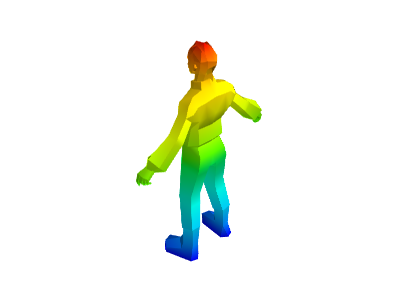
\includegraphics[width=0.19\columnwidth]{Figures/shape_retrieval/pic_person_solid.png} &
 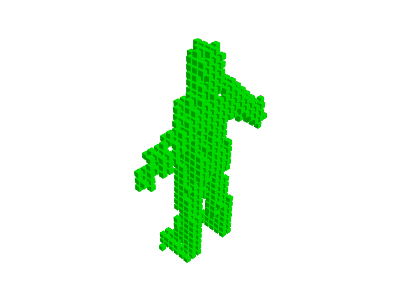
\includegraphics[width=0.19\columnwidth]{Figures/shape_retrieval/pic_person_30_solid.png} &
 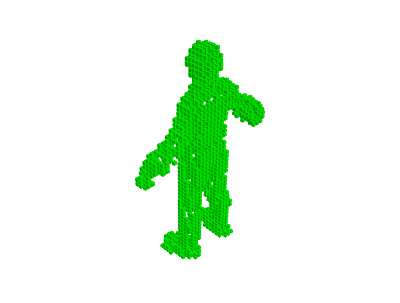
\includegraphics[width=0.19\columnwidth]{Figures/shape_retrieval/pic_person_50_solid.png} &
 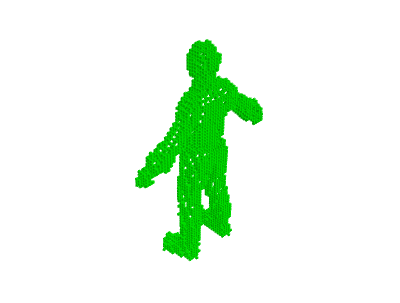
\includegraphics[width=0.19\columnwidth]{Figures/shape_retrieval/pic_person_70_solid.png} &
 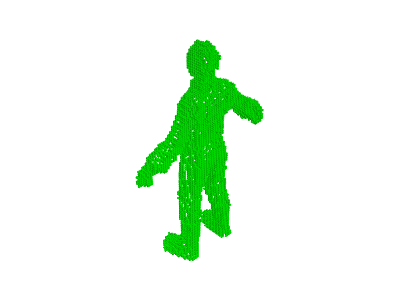
\includegraphics[width=0.19\columnwidth]{Figures/shape_retrieval/pic_person_100_solid.png} \\

 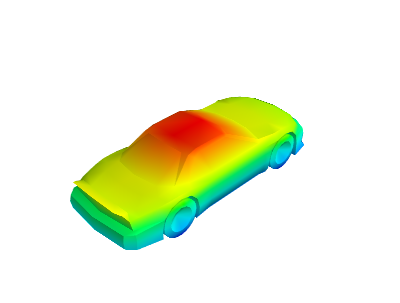
\includegraphics[width=0.19\columnwidth]{Figures/shape_retrieval/pic_car_solid.png} &
 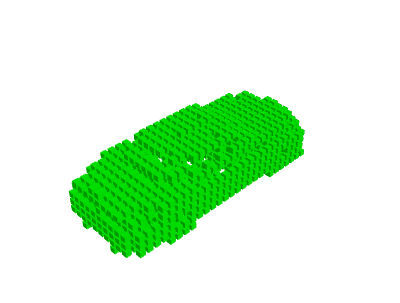
\includegraphics[width=0.19\columnwidth]{Figures/shape_retrieval/pic_car_30_solid.png} &
 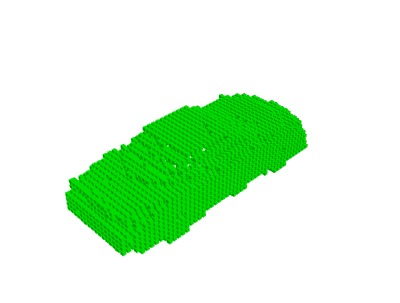
\includegraphics[width=0.19\columnwidth]{Figures/shape_retrieval/pic_car_50_solid.png} &
 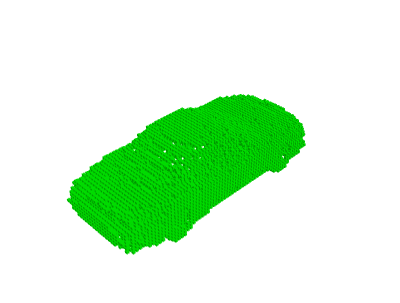
\includegraphics[width=0.19\columnwidth]{Figures/shape_retrieval/pic_car_70_solid.png} &
 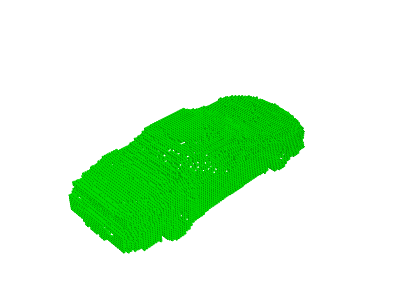
\includegraphics[width=0.19\columnwidth]{Figures/shape_retrieval/pic_car_100_solid.png} \\
\end{tabular}
\caption{Examples of some objects voxelizations at different resolutions $30$, $50$, $70$, $100$ (from left to right), left-most objects are depicted using original meshes}
\label{fig:voxels-examples}
\end{figure}


We train Sparse 3D Convolutional Neural Network (S3DCNN) on the 3D shape classification dataset by splitting it into  training and validation subsets, adding augmentation of data to achieve rotational and translational invariance. After training a model on a dataset of pairs, we use it to embed voxel representations of 3D meshes into $192$-dimensional space. The retrieval consist of ranking search objects by a cosine distance of vectors from a query vector.

The most popular metrics for evaluating retrieval performance are
\begin{itemize}
\item Precision-Recall Curve shows a trade-off between these two measures and how quickly the precision drops with the recall increase,
\item Mean average precision (mAP). Given a query, its average precision is the average of all precision values computed on all relevant objects in the retrieved list. Given several queries, the mean average precision (mAP) is the mean of average precisions for these queries. 
\end{itemize}
We evaluated mAP for different voxel rendering sizes of 3D shapes both at train and test times, see also Figure~\ref{fig:voxels-examples}.

To check if our model is comparable with other architectures, we consider a classification task. So, we trained our model for the classification task using the ModelNet40 train subset with 
\begin{itemize}
\item SoftMax last layer for $200$ epochs,
\item with exponentially discounting learning rate,
\item and performed retrieval evaluation on the test subset,
\item taking $20$ images from every class, and ranking them w.r.t their $L2$-norm by activations taken from the $17$-th layer.
\end{itemize}

Results of these experiments are provided in Table~\ref{tab:classification}. We can see that in case of classification task setup our model is comparable in terms of the classification accuracy, but mAP values are worse. But in case of metric learning performace of S3DCNN on mAP metric is much better.
Superior performance of retrieval task with MVCNN is not a surprising result, since MVCNN uses neural nets, pre-trained on ImageNet. On the other hand our model only requires 3D Shape dataset to learn.

In Figure~\ref{fig:map_for_rs} we provide the dependence of mAP on the input spatial resolution. We can see that the retrieval performance improves with increase in the input spatial resolution up to around $45-50$, after that it drops slightly and goes to plateau. It can be attributed to the insufficient amount of layers for the same scale of features, that can be separated in higher layers. Light blue color shows range of mAP on validation for top $30$ trained architectures.


\begin{figure}[!tbp]
\vspace{-20pt}
\centering
\begin{minipage}[b]{0.45\textwidth}
  \centering
  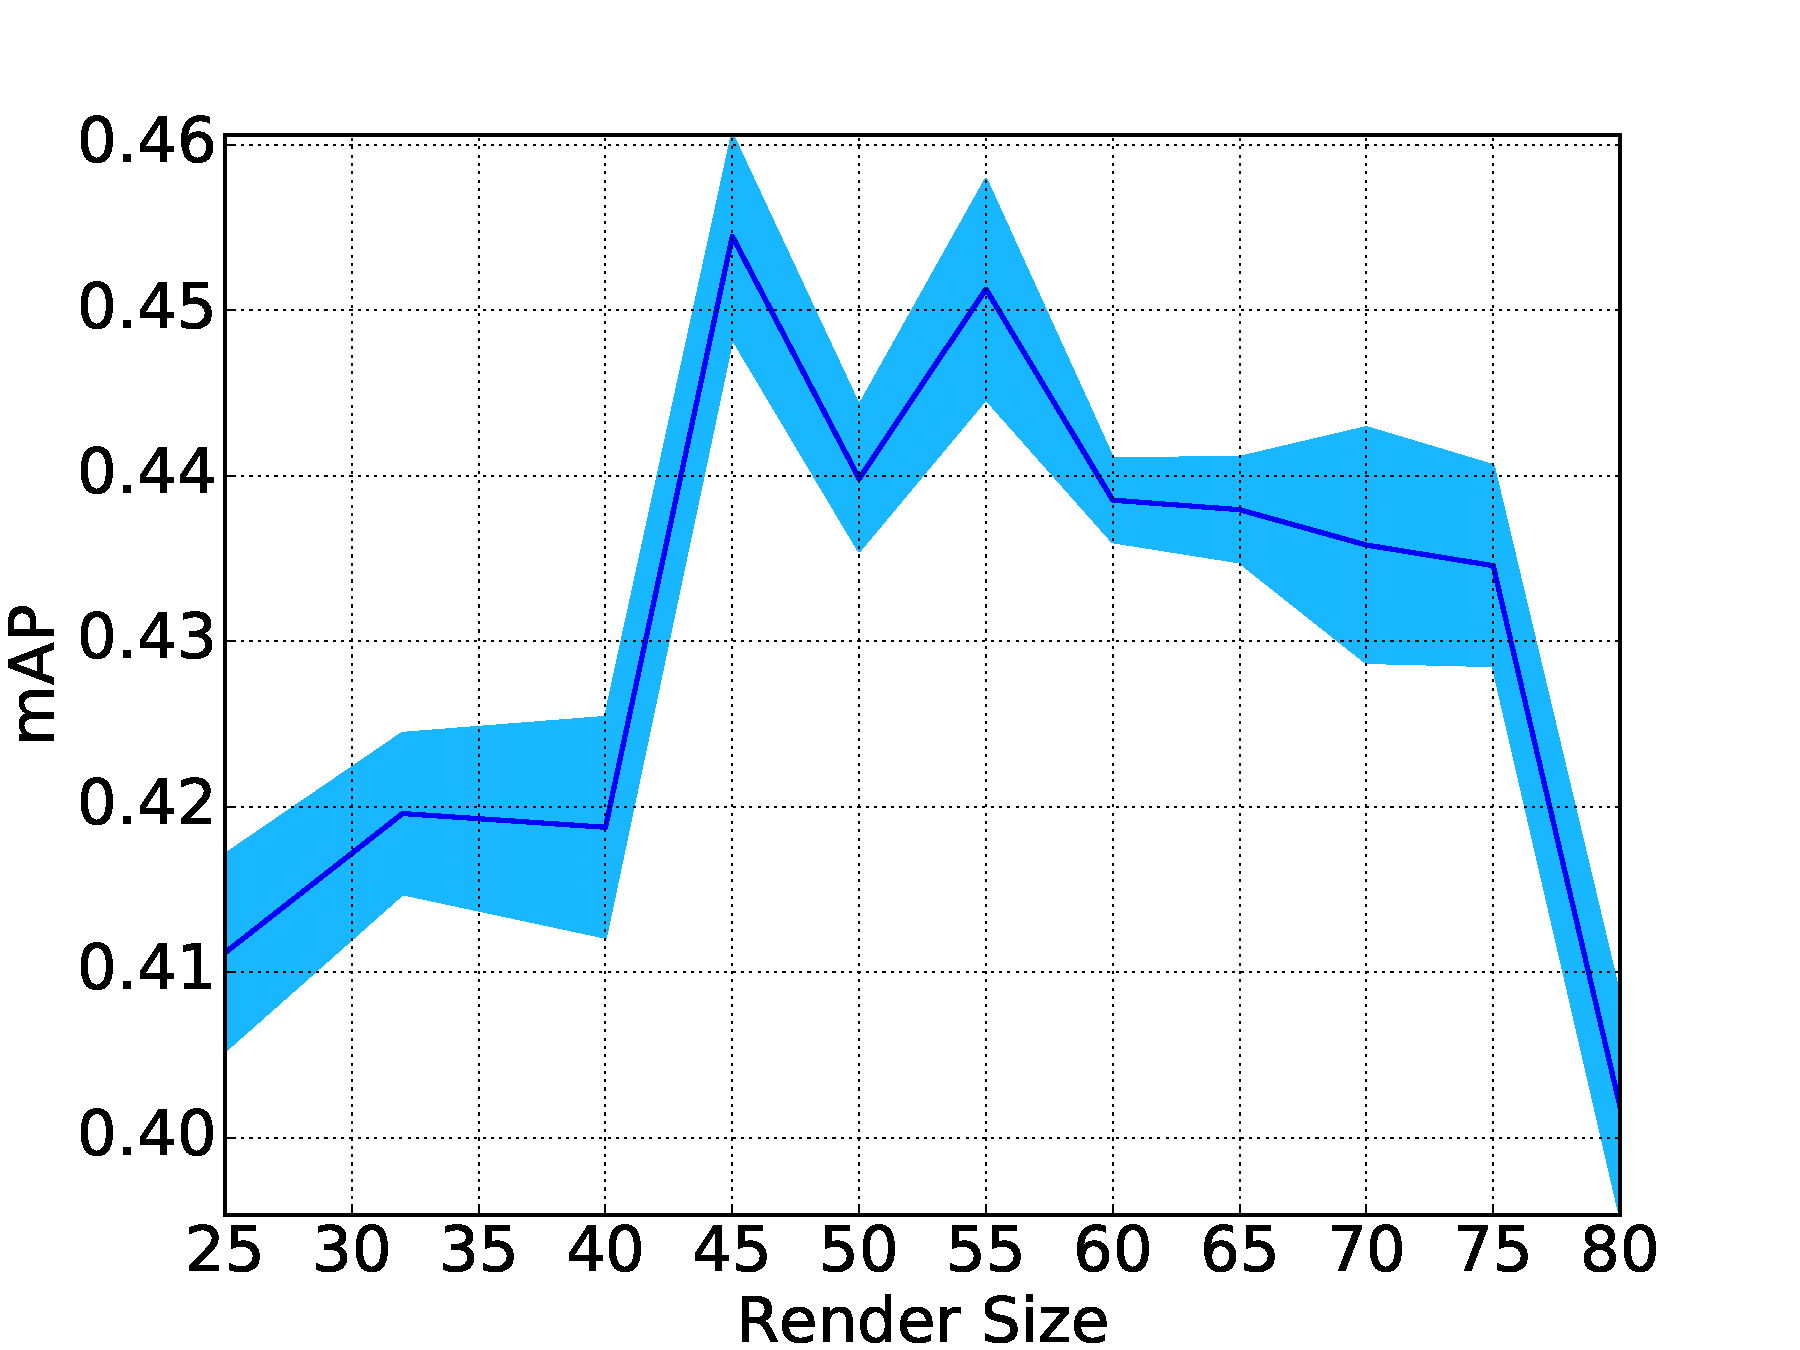
\includegraphics[width=\columnwidth]{Figures/shape_retrieval/new_map_to_rs.pdf}
  \caption{Dependence of the retrieval performance on the input spatial resolution}
  \label{fig:map_for_rs}
\end{minipage}
\begin{minipage}[b]{0.45\textwidth}
  \centering
  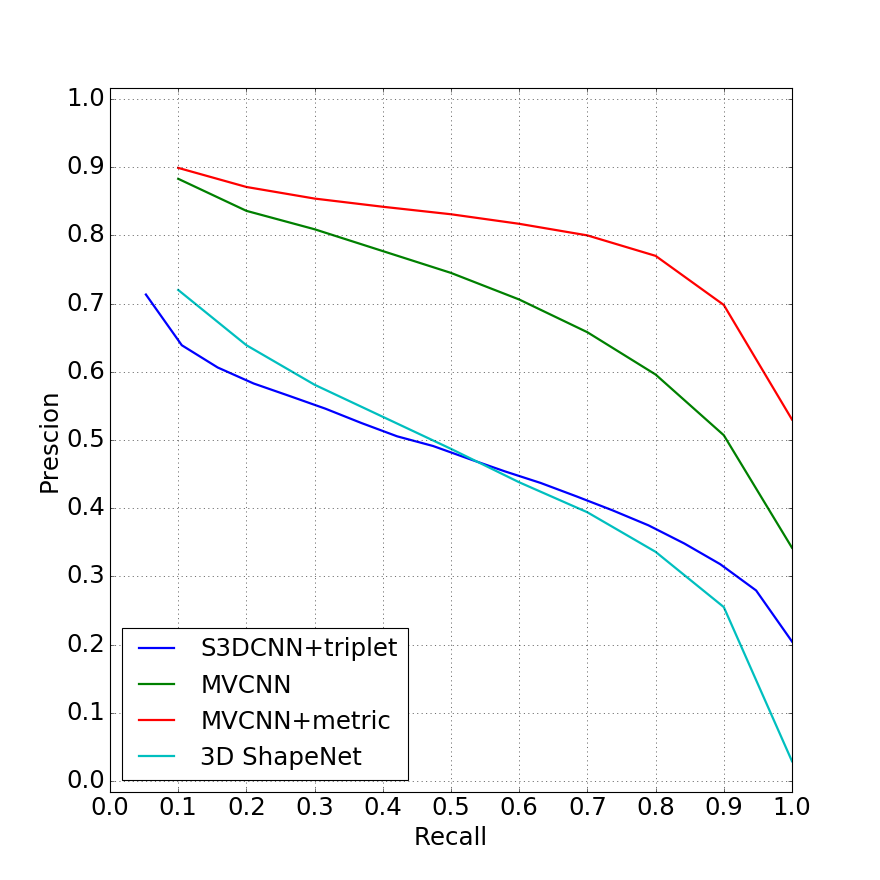
\includegraphics[width=\columnwidth]{Figures/shape_retrieval/pr_curves_comp}
  \caption{Precision-Recall curve for our method}
  \label{fig:pr_curve}
\end{minipage}
\end{figure}


We would like to note that in Figure~\ref{fig:map_for_rs} mAP values provided for different validation epochs and variability of best model can be explained by difference in total learning time.

% \begin{itemize}
% \item In Table~\ref{tab:classification} for the retrieval we used features from the last but one layer of the network,
% \item In Figure~\ref{fig:map_for_rs} we used learning with the triplet loss, for which we still have to better adjust the architecture and learning rate schedule.
% \end{itemize}
